\chapter{Aufbau und Struktur M1 Modell} \label{M1Modell}
Beim M1-Modell handelt es sich um die direkte Darstellung der zu generierenden
Objekte. Dieses Modell wird direkt durch den Generator, siehe Abschnitt
\ref{Generator}, in Quellcode umgesetzt und dient somit als Grundlage des
zu generierenden Projektes. In dem, in dieser Arbeit, beschriebenen Generator,
ist es nicht vorgesehen ein Projekt vollständig, mit allen Einzelheiten, zu
modellieren und erzeugen zu können, aus diesem Grund ist auch das M1-Modell nicht
als vollständige Abbildung für das Projekt zu verstehen, das Ziel lag vor allem
darauf die Architektur mit möglichst wenig aufwand für den Entwickler zu
generieren.

In dieser Arbeit, soll der Generator aus dem M1-Modell, eine möglichen
Grundstruktur für ein GWT-Projekt erzeugen, welches dur kleine änderunge
lauffähig ist. Das M1-Modell ist so angedacht, dass alle Seiten eine
eigenständige Klasse darstellen. Des Weiteren können einfache Elemente, wie
u. A. Label und Textfelder den Seiten hinzugefügt werden.
Zu dem ist es möglich die Navigation zwischen den Seiten, beispielsweise mit
Hilfe eines Menüs, in das Modell mit einzubringen. 

Durch die Verwendung eines Profils sind in dem M1-Modell keine Assoziationen
zu sehen. Dies sorg dafür, dass keine Verbindung zwischen den einzelnen Seiten
zu sehen ist. Die Navigation wird ausschließlich über die Properties der
Navigations Elemente erstellt, in dieser Arbeit mit
\texttt{viewNavigationObject} benannt. Dies sorgt für eine leichtere Erstellung
dessen Im M1-Modell durch den Entwickler, erschwert allerdings das Erkennen
der Navigation.

\section{M1-Modellaufbau}
Wenn ein neues Projekt angelegt wird, muss in den Properties des M1-Modells
neben der Angabe des Profils, ein Name definiert werden. Dieser Name stellt
später den Hauptpaketnamen des GWT-Projektes dar und legt somit den Grundstein
für die Paketstruktur (siehe Abbildung \ref{Fig:mainpackage}).

\begin{figure}[htbp]
\begin{center}
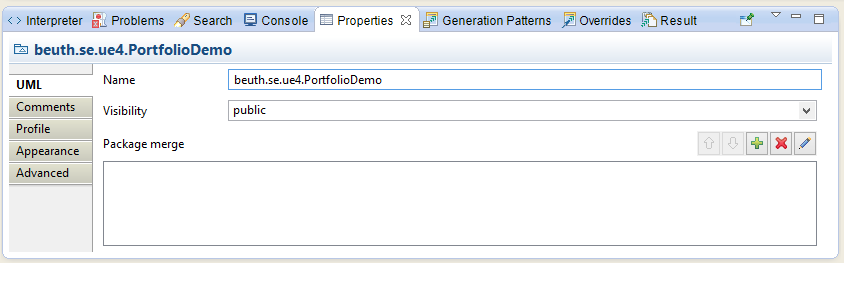
\includegraphics[width=0.8\textwidth]{./img/ProjectPackage.png}
\caption{Name des Modelles und gleichzeitig Hauptpaket des
GWT-Projekts}\label{Fig:mainpackage}
\end{center}
\end{figure}

\newpage
\section{Klassenaufbau}
Die grundlegendsten Elemente in dem Modell sind \texttt{ViewImpl}-Klassen. Ein
Beispiel dafür ist in Abbildung \ref{Fig:viewimpl} zu sehen. Für jede dieser
Klassen-Objekte werden mithilfe des Generators alle notwendigen Dateien
erzeugt, die für den späteren Seiteaufruf notwendig sind.

\begin{figure}[htbp]
\begin{center}
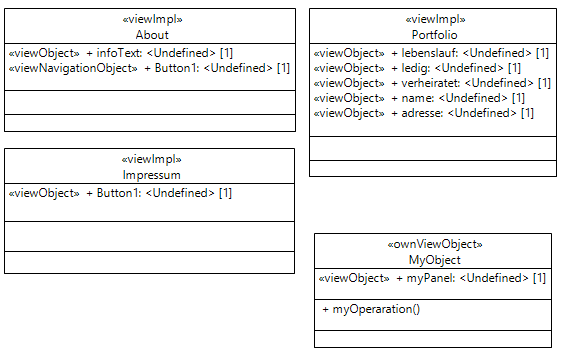
\includegraphics[width=1.0\textwidth]{./img/GWT-Model-Views-alg.png}
\caption{\texttt{ViewImpl}-Klassen zur Erzeugung von Seiten
für den Webauftritt.}\label{Fig:viewimpl}
\end{center}
\end{figure}

Des Wietern ist in der Abbildung \ref{Fig:viewimpl} ein Beispiel für ein
\texttt{ownViewObject} zu sehen. Diese sind für komplexere oder mehrfach
verwendete UI-Struckturen gedacht und werden vom Generator als eigenständige
Klasse generiert.

GWT bietet, durch Verwendung des MVP-Pattern, eine einfache Möglichkeit Seiten
auszutauschen. Um dieses Verfahren mit zu generieren wurde sich dazu
entschlossen, neben der Standardgenerierung von Seiten, eine zusätzliche
Methode einzubauen. Diese Methode bietet die Möglichkeit beliebig viele
alternativ Seiten für eine Ansicht im Webauftritt zu erzeugen (siehe Abbildung
\ref{Fig:viewInterface}). Die Möglichkeit der einfachen Austauschbarketi von
Views, wurde bei GWT unter anderem für Testzwecke angedacht.

\begin{figure}[htbp]
\begin{center}
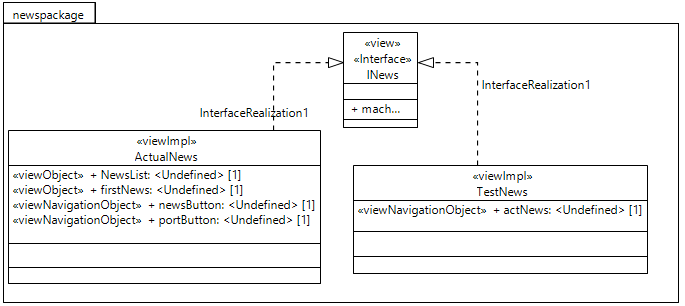
\includegraphics[width=1.0\textwidth]{./img/GWT-Model-Views-interface.png}
\caption{Ein Beispiel für die Verwendung der \texttt{ViewInterface}-Klassen
um mit Hilfe einer Vielzahl von \texttt{ViewImpl}-Klassen
eine austauschbare Ansicht zu erzeugen.}\label{Fig:viewInterface}
\end{center}
\end{figure} 

Bei dem, in Abbildung \ref{Fig:viewInterface}, gezeigtem M1-Modell Ausschnitt
wird die Komplette Klassenstruktur nicht zweimal erzeugt, anders als im
allgemeinem Fall (siehe Abbildung \ref{Fig:viewimpl}). Die
\grqq{}Name\grqq{}Activity.java, \grqq{}Name\grqq{}Place.java und
\grqq{}Name\grqq{}View.java Klassen werden hierbei nur einmal für das Interface
und die \grqq{}Name\grqq{}ViewImpl.java und \grqq{}Name\grqq{}ViewImpl.ui.xml
Dateien für jede realisierende \texttt{ViewImpl}-Klassen generiert. 

Darüber hinaus ist in Abbildung \ref{Fig:viewInterface} zu sehen, dass es
möglich ist, Klassen zu Paketen zuzuordnen. Auf diese Weise wird es
ermöglicht die zu generierenden Dateien zu gruppieren. 

\newpage
Das letzte in dem Modellen genutzte Klassenkonstrukt, sind die sogenannten
\texttt{PermanentView}-Elemente. Diese sind dazu gedacht, um zum Beispiel Menüs
zu erzeugen. Diese haben die Eigenschaft das sie auf allen Seiten zur Verfügung
stehen und nicht mehrfach generiert werden sollen.

\begin{figure}[htbp]
\begin{center}
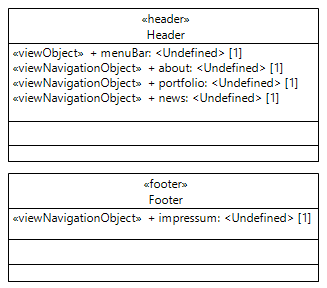
\includegraphics[width=0.55\textwidth]{./img/Header_Footer.png}
\caption{\texttt{PermanentView}-Elemente am Beispiel
eines Headers, mit Menu, und eines Footers.}\label{Fig:headerFooter}
\end{center}
\end{figure} 

\newpage
\section{Seitenaufbau}
Je nach Art der Seite muss zuerst definiert werden, um was für einen Typ von
Seite es sich handelt. In Abbildung \ref{Fig:SideProp} ist ein Beispiel dafür
zu sehen, welches eine \texttt{ViewImpl} und ein \texttt{Header} zeigt, eine
spezialisierte Form der \texttt{PermanentView}, zu sehen. Wichtig ist hier
die "`concreteBinding"' Eigenschaft. An dieser Stelle kann bei Verwendung eines
separaten Interfaces festgelegt werden, welche konkrete implementierung
dargestellt werden soll, um keine Laufzeitfehler zu erzeugen muss zu jeder View
exakt eine ViewImpl angegeben werden. Diese Einstellung kann später im
Quellecode geändert werden.

\begin{figure}[htbp]
\begin{center}
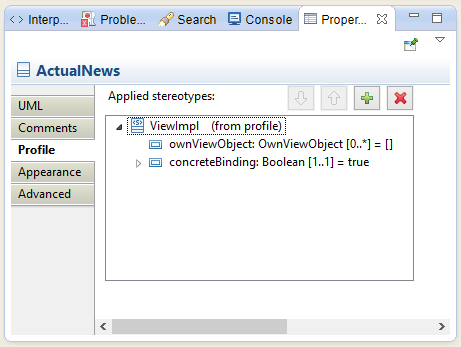
\includegraphics[width=0.8\textwidth]{./img/Prop-ViewImp.png}
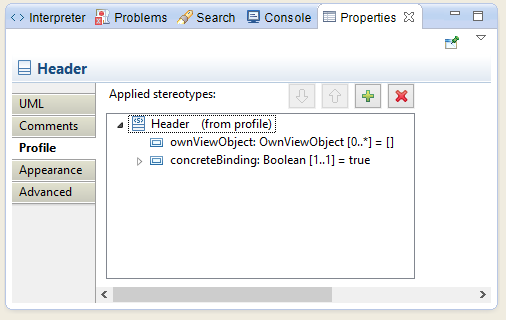
\includegraphics[width=0.8\textwidth]{./img/Prop-Header.png}
\caption{Klassen mit definierten Stereotypen, oben
eine \texttt{ViewImpl} und unten ein \texttt{Header}}\label{Fig:SideProp}
\end{center}
\end{figure} 

Um diese Seite mit Inhalten zu befüllen, können \texttt{ViewObject}s und 
\texttt{ViewNavigationObject}s als Attribute hinzugefügt werden.

Bei \texttt{ViewObject}-Elementen können die in Abbildung \ref{Fig:ViewProp}
dargestellten Eigenschaften verändert werden.

\begin{figure}[htbp]
\begin{center}
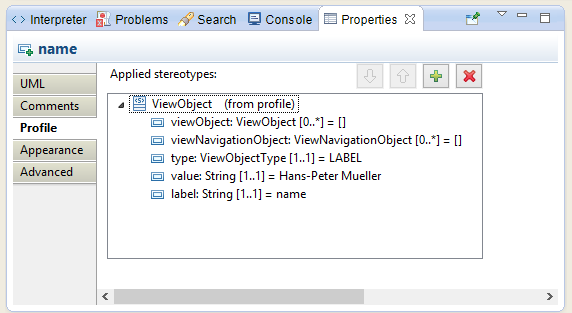
\includegraphics[width=0.8\textwidth]{./img/Prop-ViewObjects.png}
\caption{Eigenschaften eines \texttt{ViewObject}-Elementes }\label{Fig:ViewProp}
\end{center}
\end{figure} 

Bei \texttt{ViewNavigationObject}-Elementen können die in Abbildung
\ref{Fig:ViewNavProp} dargestellten Eigenschaften verändert werden. Hier ist
vor allem die letzte Eigenschaft "`goToView"' zu beachten, welche angibt wohin
dieses navigieren soll.

\begin{figure}[htbp]
\begin{center}
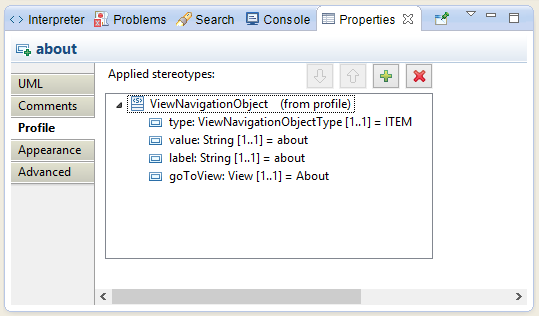
\includegraphics[width=0.8\textwidth]{./img/Prop-ViewNavigationObjects.png}
\caption{Eigenschaften eines \texttt{ViewNavigationObject}-Elementes
}\label{Fig:ViewNavProp}
\end{center}
\end{figure}
